\documentclass[11pt]{article}
\usepackage[T1]{fontenc}
\usepackage[margin=0.94in]{geometry}
\usepackage{amsmath,amssymb,amsthm,mathtools}
\usepackage{graphicx}
\usepackage{microtype}
\usepackage{xcolor}
\usepackage[hypertexnames=false,colorlinks=true,linkcolor=blue!55!black,urlcolor=blue!65!black,citecolor=blue!55!black]{hyperref}

\newtheorem{theorem}{Theorem}
\newtheorem{lemma}[theorem]{Lemma}
\newtheorem{remark}[theorem]{Remark}
\newcommand{\R}{\mathbb R}
\newcommand{\Hh}{\mathbb H}
\newcommand{\Ptwo}{\mathcal P_2}
\newcommand{\Ua}{\mathcal U_\alpha}
\newcommand{\Uat}{\widetilde{\mathcal U}_\alpha}
\newcommand{\supp}{\operatorname{supp}}
\newcommand{\Law}{\operatorname{Law}}
\newcommand{\ip}[2]{\left\langle #1,#2\right\rangle}

\title{The \(C^{1,\alpha}\) Wasserstein--Hilbert lift\\
equivalence fails for every \(0<\alpha<1\)}
\author{Candidate full counterexample to Remark 3.12(i) of arXiv:2004.01660}
\date{12 August 2026}

\begin{document}
\maketitle

\noindent
\fbox{\begin{minipage}{0.94\textwidth}
\textbf{Status: candidate full counterexample, likely valid.}
For every \(0<\alpha<1\), there is a continuously differentiable
\(\Ua:\Ptwo(\R)\to\R\) whose rearrangement-invariant lift
\(\Uat:L^2(\Omega)\to\R\) is globally \(C^{1,\alpha}\), while \(\Ua\) is
not \(C^{1,\alpha}\) in Definition 3.8 of Gangbo--M\'esz\'aros.
The example is the \((1+\alpha)\)-power of the second-moment radius.
It even satisfies the definition's optimal-transport Taylor estimate;
only the required pointwise H\"older regularity on a measure's support
fails. Thus the proposed equivalence is false.
\end{minipage}}

\section{The exact open problem}

Let \(\Omega\) be an atomless probability space and
\(\Hh=L^2(\Omega;\R)\). The source lifts a functional
\(\mathcal U:\Ptwo(\R)\to\R\) by
\[
 \widetilde{\mathcal U}(X)=\mathcal U(\Law(X)).
\]
Its Definition 3.8 says, in particular, that
\(\mathcal U\in C^{1,\alpha}\) only if there is one constant \(C\) such
that, for every \(\mu\),
\begin{equation}
 |\nabla_w\mathcal U(\mu)(q)-\nabla_w\mathcal U(\mu)(r)|
 \le C|q-r|^\alpha
 \qquad(q,r\in\supp\mu).
 \tag{1}
\end{equation}
It also requires the first-order remainder along every optimal coupling
to be \(O(W_2^{1+\alpha})\).

Lemma 3.11 of the source proves equivalence between its Wasserstein
\(C^{1,1}\) class and the ordinary Hilbert \(C^{1,1}\) class. Remark
3.12(i) asks whether the equivalence persists for
\(C^{1,\alpha}\), \(0<\alpha<1\) \cite{GM}. The complete source pages
containing Definition 3.8 and the question are reproduced next.

\begin{center}
 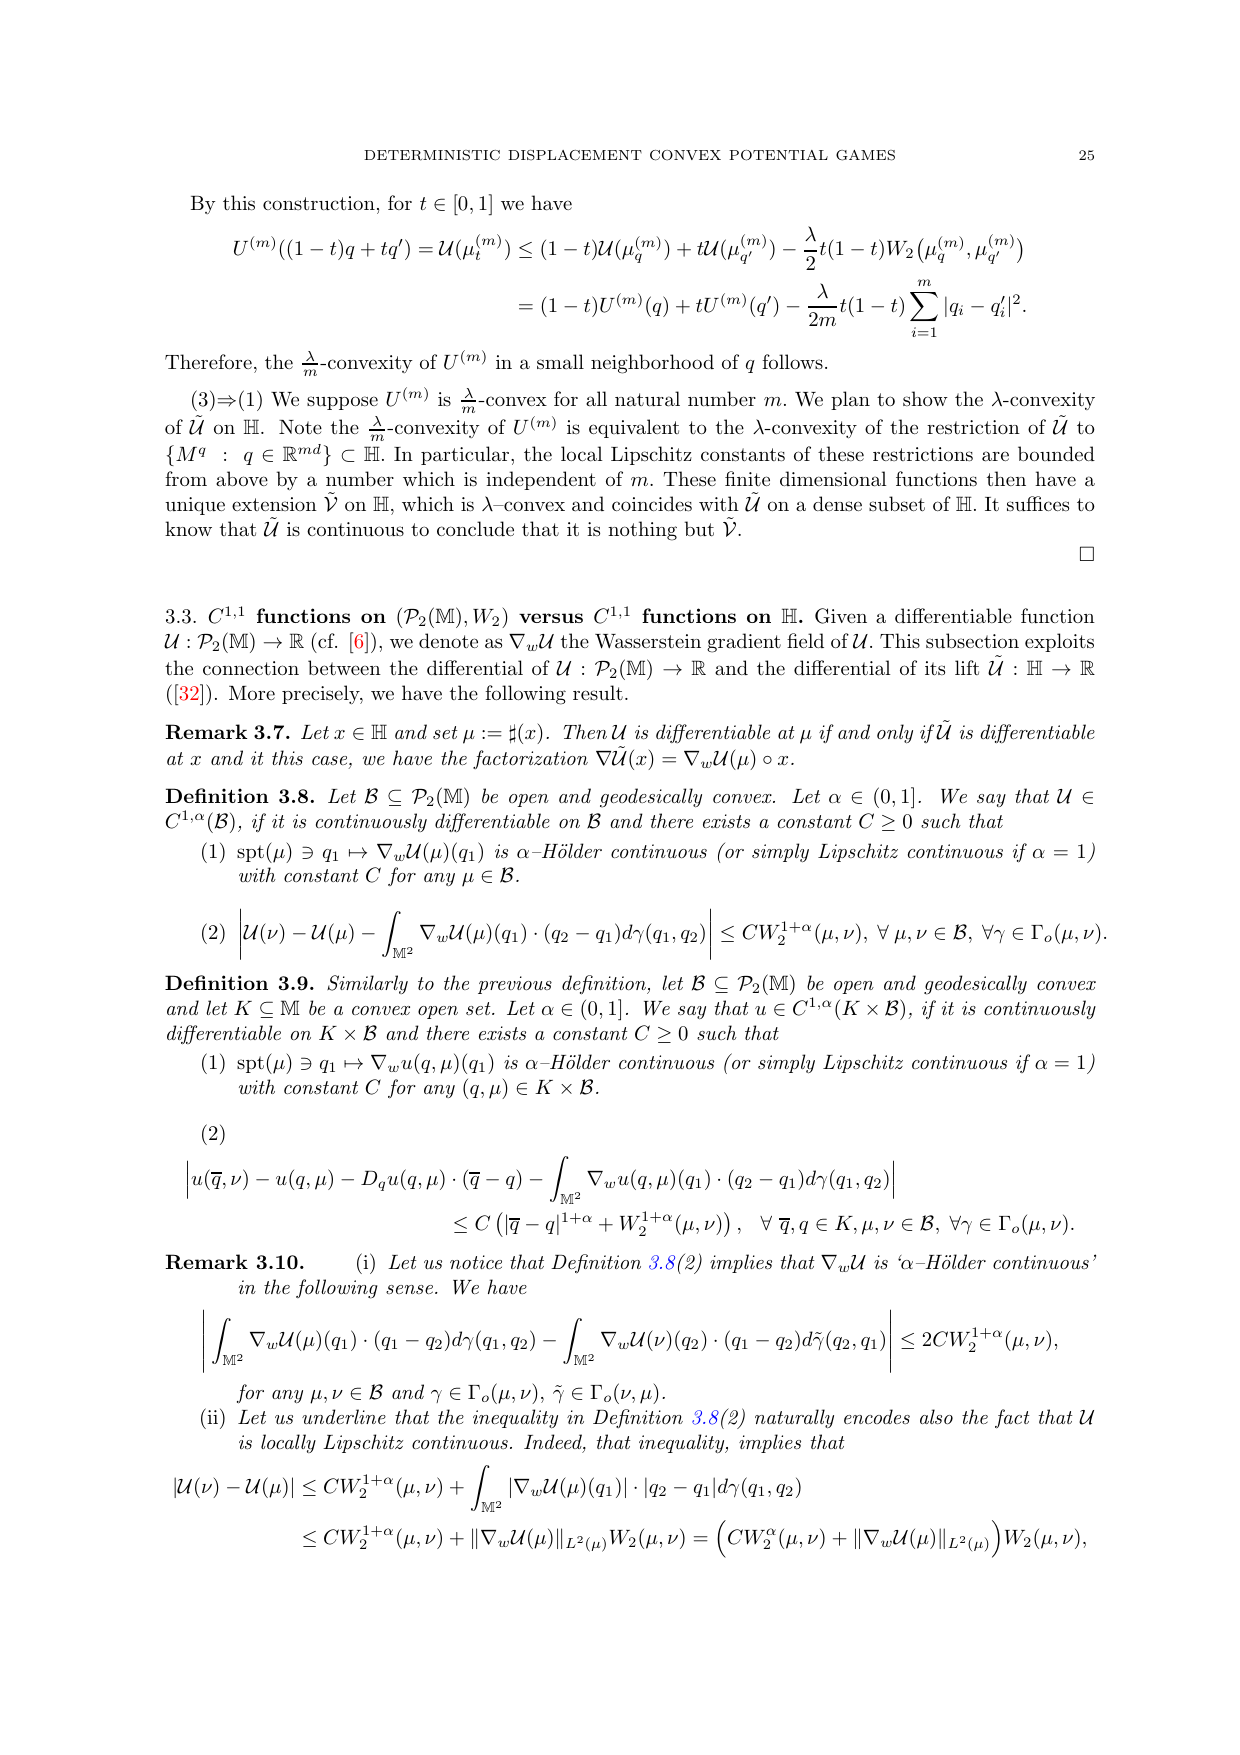
\includegraphics[height=0.78\textheight]{figures/source_page25-25.png}
\end{center}

\clearpage

\begin{center}
 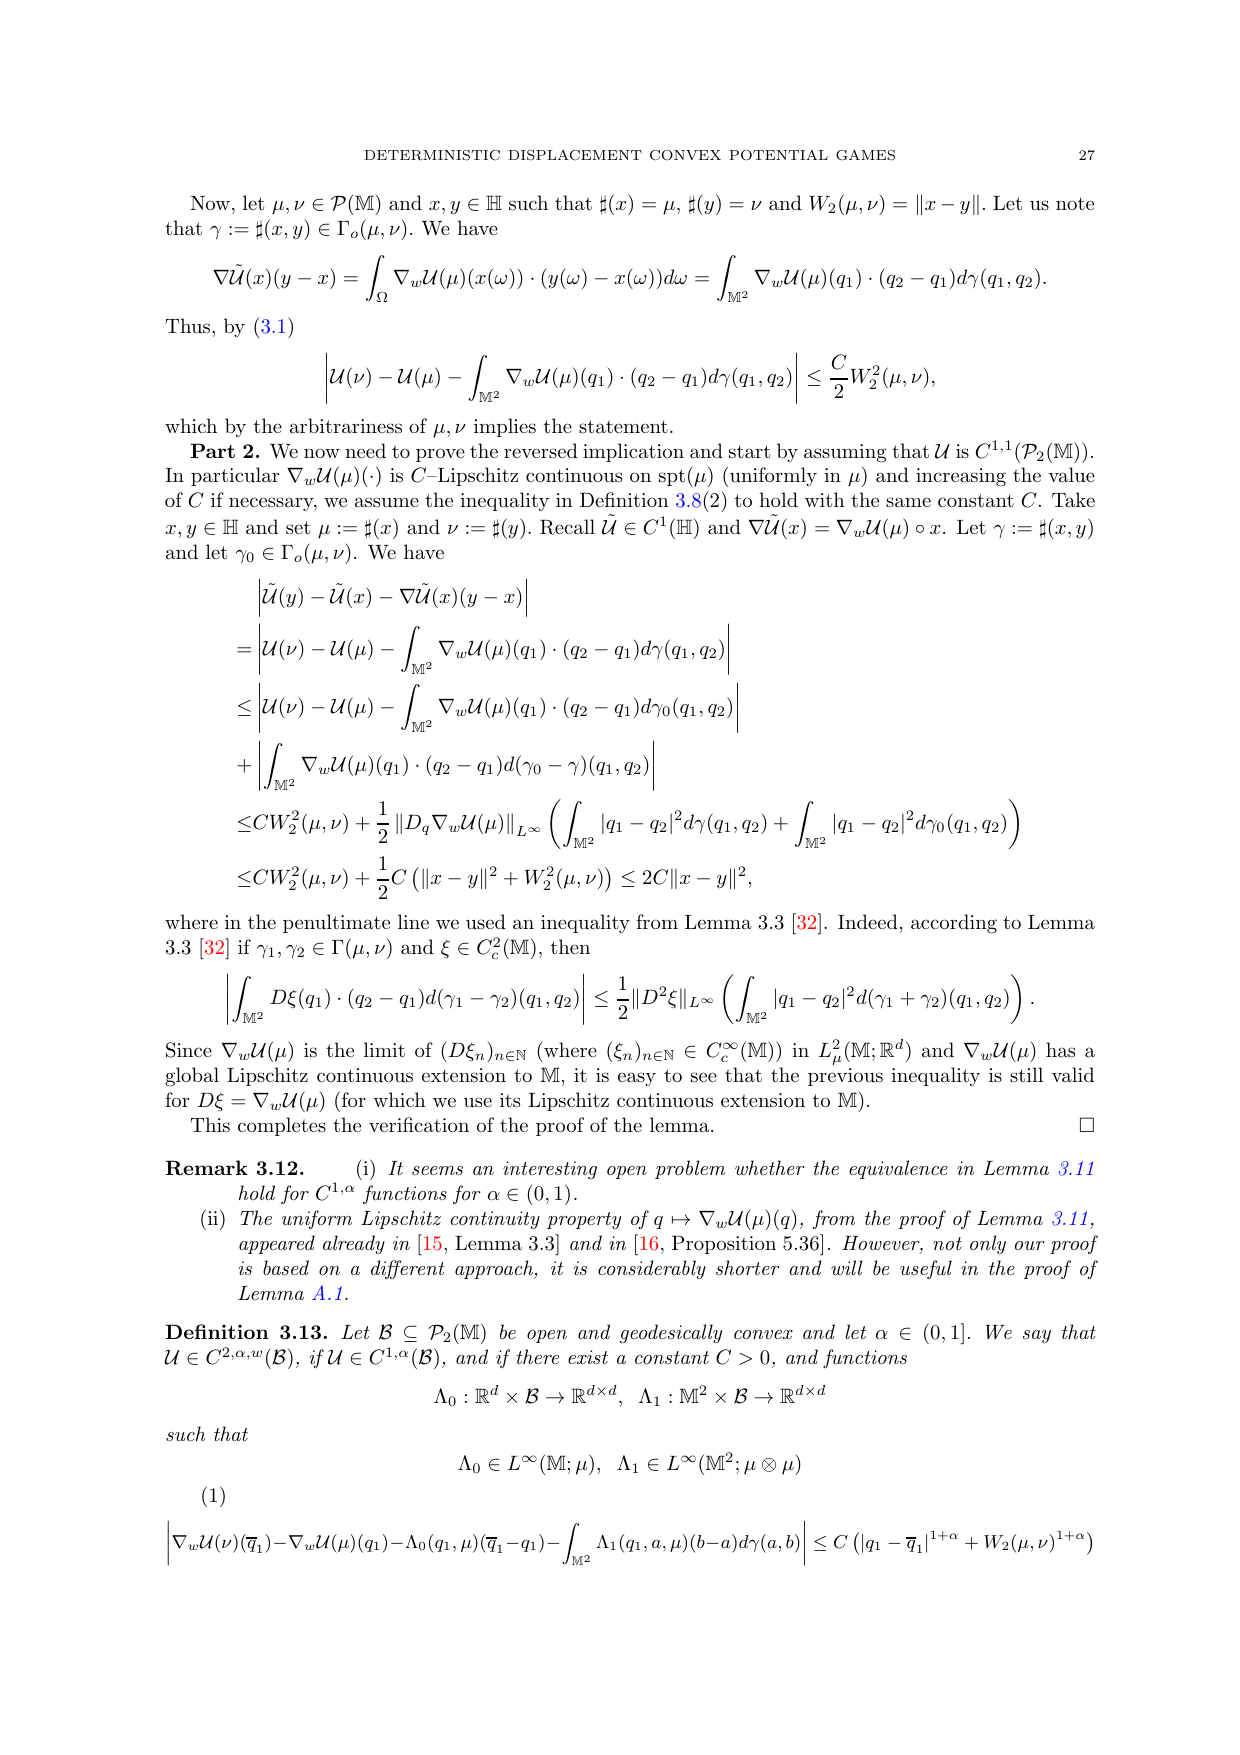
\includegraphics[height=0.78\textheight]{figures/source_page27-27.png}
\end{center}

\section{The counterexample}

Fix \(0<\alpha<1\). For \(\mu\in\Ptwo(\R)\), write
\[
 m_2(\mu)=\int_{\R}q^2\,d\mu(q)
\]
and define
\begin{equation}
 \Ua(\mu)=\frac{1}{1+\alpha}\,
             m_2(\mu)^{(1+\alpha)/2}.
 \tag{2}
\end{equation}

\begin{theorem}\label{thm:main}
The lift of \(\Ua\) belongs to \(C^{1,\alpha}(\Hh)\), globally. The
functional \(\Ua\) is continuously Wasserstein differentiable and obeys
the \(O(W_2^{1+\alpha})\) Taylor-remainder clause in Definition 3.8.
Nevertheless, it violates the supportwise H\"older clause \emph{(1)}.
Consequently the \(C^{1,\alpha}\) equivalence in Remark 3.12(i) is false
for every \(\alpha\in(0,1)\).
\end{theorem}

The Hilbert estimate behind the example is elementary.

\begin{lemma}\label{lem:holder}
On any real Hilbert space \(H\), the map
\[
 J_\alpha(z)=
 \begin{cases}
 \|z\|^{\alpha-1}z,&z\ne0,\\
 0,&z=0,
 \end{cases}
\]
satisfies
\[
 \|J_\alpha(x)-J_\alpha(y)\|\le3\|x-y\|^\alpha
 \qquad(x,y\in H).
 \tag{3}
\]
\end{lemma}

\begin{proof}
Set \(r=\|x\|\), \(s=\|y\|\), and \(d=\|x-y\|\), and suppose
\(r\ge s>0\); the cases with a zero vector are immediate. With
\(\widehat x=x/r\) and \(\widehat y=y/s\),
\[
 \|J_\alpha(x)-J_\alpha(y)\|
 \le r^\alpha-s^\alpha+s^\alpha
      \|\widehat x-\widehat y\|.
\]
Concavity gives \(r^\alpha-s^\alpha\le(r-s)^\alpha\le d^\alpha\).
Also
\[
 \|\widehat x-\widehat y\|
 \le \frac d r+\frac{r-s}{r}\le\frac{2d}{r}.
\]
If \(d\le r\), the second term is at most
\(2r^{\alpha-1}d\le2d^\alpha\). If \(d>r\), it is at most
\(2s^\alpha\le2r^\alpha<2d^\alpha\). This proves (3).
\end{proof}

\section{Verification of every hypothesis}

If \(X\in\Hh\), then (2) lifts to the radial functional
\begin{equation}
 \Uat(X)=\frac{1}{1+\alpha}\|X\|_2^{1+\alpha}.
 \tag{4}
\end{equation}
It is Fr\'echet differentiable everywhere and
\[
 \nabla\Uat(X)=J_\alpha(X).
 \tag{5}
\]
Lemma \ref{lem:holder} therefore proves the asserted global
\(C^{1,\alpha}\) regularity. It also gives the explicit Taylor estimate
\begin{align}
 \big|\Uat(Y)-\Uat(X)-\ip{J_\alpha(X)}{Y-X}\big|
 &\le \int_0^1
 \|J_\alpha(X+t(Y-X))-J_\alpha(X)\|_2\|Y-X\|_2\,dt \notag\\
 &\le \frac{3}{1+\alpha}\|Y-X\|_2^{1+\alpha}.
 \tag{6}
\end{align}

Now let \(X\) have law \(\mu\). The derivative in (5) factors through
\(X\), so the Wasserstein gradient is
\begin{equation}
 \nabla_w\Ua(\mu)(q)=
 \begin{cases}
 m_2(\mu)^{(\alpha-1)/2}q,&m_2(\mu)>0,\\
 0,&m_2(\mu)=0.
 \end{cases}
 \tag{7}
\end{equation}
This field is a gradient in \(q\), hence belongs to the Wasserstein
tangent space. Its continuity also follows directly: if
\(\mu_n\to\mu\) in \(W_2\), choose optimal lifts
\(X_n\to X\) in \(L^2\); then (3) gives
\[
 \|J_\alpha(X_n)-J_\alpha(X)\|_2
 \le3\|X_n-X\|_2^\alpha\longrightarrow0.
\]
Thus \(\Ua\) is continuously Wasserstein differentiable, including at
\(\delta_0\).

Moreover, for any optimal coupling \(\gamma=\Law(X,Y)\), the linear
term in (6) is
\[
 \ip{J_\alpha(X)}{Y-X}
 =\int_{\R^2}\nabla_w\Ua(\mu)(q)(r-q)\,d\gamma(q,r),
\]
and \(\|X-Y\|_2=W_2(\mu,\nu)\). Hence (6) is precisely the
\(O(W_2^{1+\alpha})\) clause of Definition 3.8, with constant
\(3/(1+\alpha)\).

\section{The decisive failure}

Take the standard Gaussian measure \(\gamma\) on \(\R\). It has
\(m_2(\gamma)=1\) and \(\supp\gamma=\R\), so (7) becomes
\[
 \nabla_w\Ua(\gamma)(q)=q.
\]
If the supportwise H\"older requirement (1) held with any finite
constant \(C\), then for every \(t>0\),
\[
 t=|\nabla_w\Ua(\gamma)(t)-\nabla_w\Ua(\gamma)(0)|
 \le Ct^\alpha,
\]
or \(t^{1-\alpha}\le C\), which is impossible as \(t\to\infty\).
No change of representative can repair this: a continuous
representative agreeing with \(q\mapsto q\) Gaussian-almost everywhere
must agree with it on all of \(\R\).

The same argument rules out a local version on any Wasserstein
neighborhood containing \(\gamma\), because the failure already occurs
for the single measure \(\gamma\). Thus it is not an artifact of asking
for a global estimate across distant probability measures. What breaks
for \(\alpha<1\) is the passage from an \(L^2\)-H\"older estimate on
rearrangements to a pointwise H\"older estimate on an unbounded support.
For \(\alpha=1\), the small-set scaling used in the source's proof is
exactly balanced; for \(\alpha<1\), it is not.

\section{Conclusion}

The answer to Remark 3.12(i) is negative for every exponent it asks
about. The counterexample is scalar, explicit, rearrangement invariant,
and globally \(C^{1,\alpha}\) on the Hilbert lift. It passes the
Wasserstein differentiability and optimal-coupling Taylor tests, while
failing only the additional supportwise regularity built into the
source's definition. Exact-phrase and citation searches found the
published source still stating the problem and no later resolution of
this specific equivalence.

\begin{thebibliography}{9}
\bibitem{GM}
W. Gangbo and A. R. M\'esz\'aros,
\emph{Global well-posedness of Master equations for deterministic
displacement convex potential mean field games},
Comm. Pure Appl. Math. \textbf{75} (2022), 2685--2801;
arXiv:2004.01660, Remark 3.12(i).
\end{thebibliography}

\end{document}
